% !TEX root =  CurvedFoldedDogs.tex

\section{Setup} \label{sec:setup}
\subsection{Definitions}
Throughout the paper, we use the following definition for a curved folded surface:
\begin{definition} \label{def:curved_folded_surface}
A surface $S$ is called a curved folded surface if it is locally isometric to the plane and can be written as $S = \bigcup P_i $ where each $P_i$ is a $C^2$ developable surfaces termed a \emph{patch}, and intersections of the patches $P_i \cap P_j$ are $C^2$ curves.
\end{definition}
% consists piecewise $C^2$ developable surface whose discontinuities are focused along $C^2$ curves. More formally, 
This definition is suitable for various topologies, such as a cylinder, but throughout this paper we work with surfaces that can be globally isometrically flattened to the plane. Borrowing terms from \cite{origami_book,non_pleated}, we often refer to the surface \emph{crease pattern} as the planar isometric surface domain $S_P$ together with the flattened intersection curves between the interior \OSH{why interior?} of the patches $P_i$ (see \figref{fig:crease_pattern}). \OSH{We could have global overlaps in principle? also, we could do holes? This all sounds like we can't. But providing a crease pattern on globally self-overlapping domain or domain with holes is just a problem of UI, not your method. Maybe we could use a similar formulation to the first paper, saying that we focus on topologies that can be seen as subsets of $\mathbb{R}^2$? Or make a comment about that in discussion section at least?} Flattened creases with nonzero curvature are said to be curved, while those with vanishing curvature are said to be straight. A crease might be partly curved and partly straight, or curved almost everywhere but with an inflection point where the curvature vanishes. When we discuss curved folds, we always assume nonzero curvature, unless specified otherwise \OSH{so, we assume NO inflection points for curved folds?}. The flattened domain boundaries together with the flattened intersection curves form a (pseudoline \OSH{is it necessary to say `pseudoline'? Arrangement is a very general thing in comp.\ geo.}) planar arrangement \cite{arrangements}, inducing a planar graph that decomposes $S_p$ into different connected components termed faces, which are domains isometric to the patches $P_i$. The vertices of this graph are the intersection points of the curves with each other or the boundary curves, which we call \emph{crease vertices}. The \emph{edges} of this graph are curves isometric to the intersections of the various patches (see \figref{fig:crease_pattern}), and we refer to the inner points of these curves as \emph{crease points}, i.e., the points on these curves that are not \textit{crease vertices}. We say that $S$ is \emph{folded} along a crease point $p$ if at that point the patches $P_i,P_j$ sharing it have a tangential discontinuity \OSH{the patches are not defined beyond the intersection curves, so they don't have a tangential discontinuity, rather, $S$ has a tangential discontinuity. Maybe say ``if at that point $S$ has a tangent discontinuity, i.e., the tangent plane of $P_i$ does not coincide with the tangent plane of $P_j$, where $P_i, P_j$ are the two patches at $p$} (see \figref{fig:folded_and_not_folded}).

\begin{figure} [h]
	\centering
	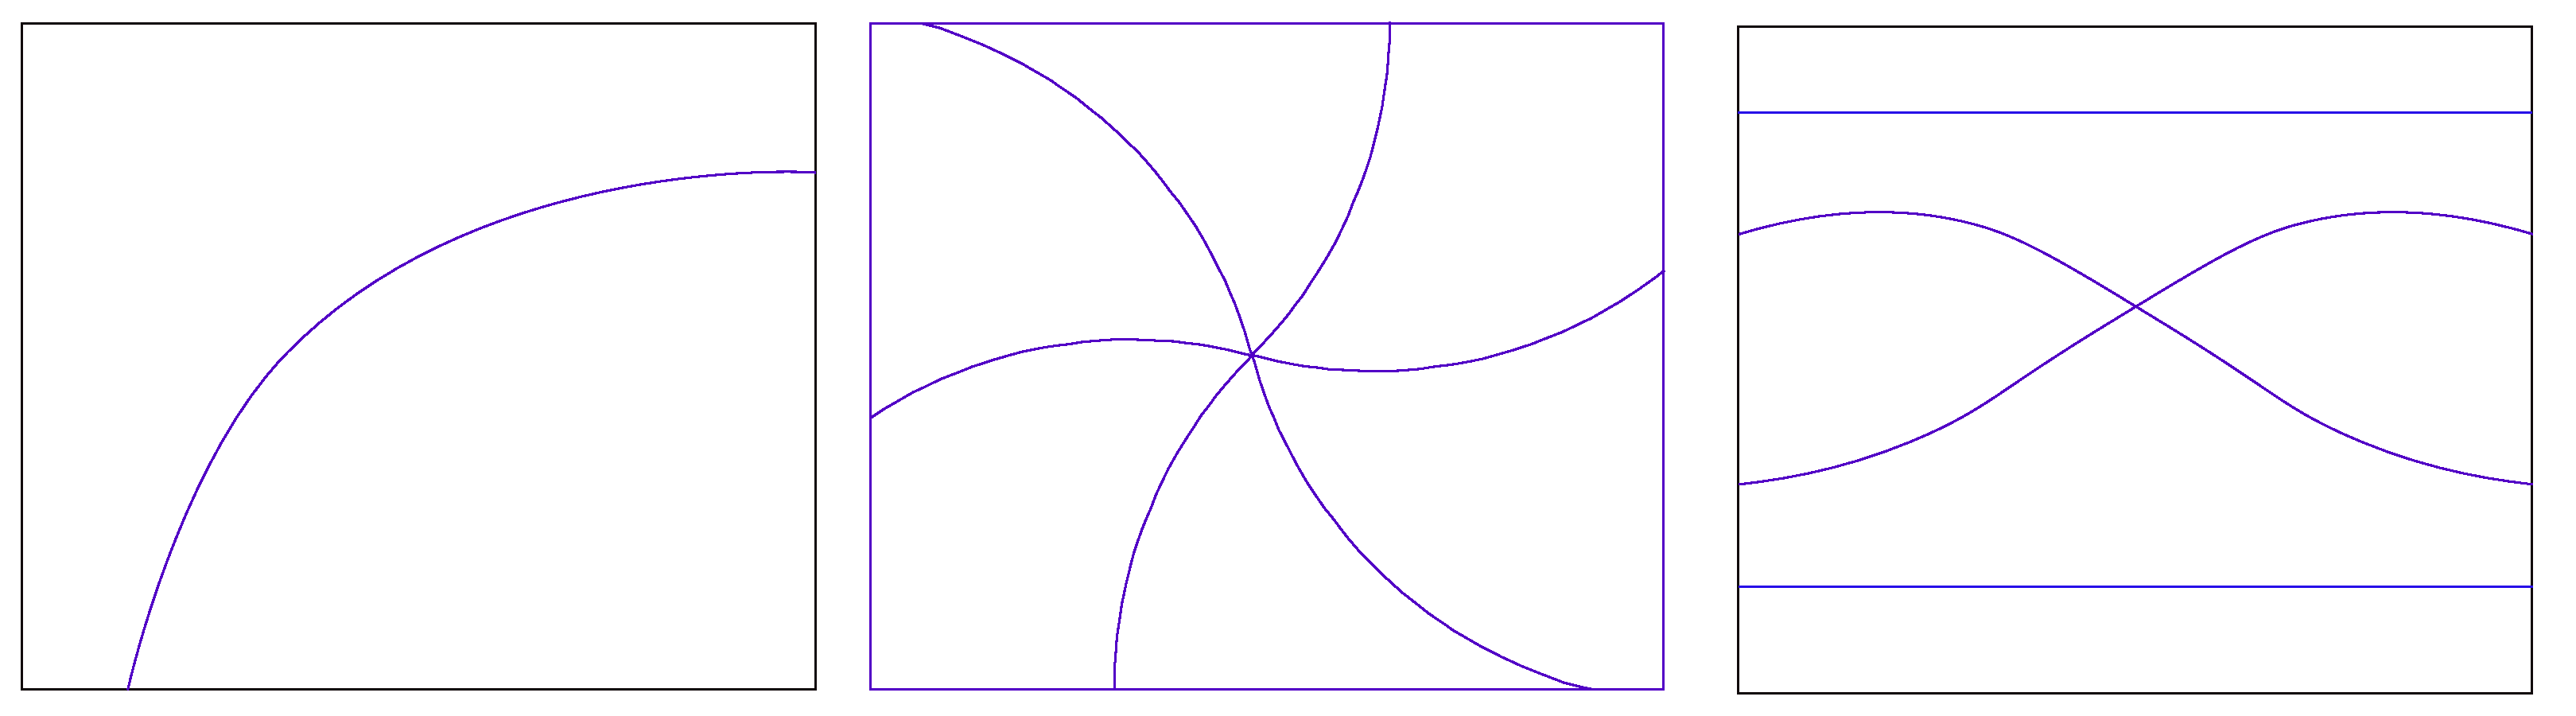
\includegraphics[width=\linewidth]{figures/crease_patterns}
	\caption{Curved crease patterns, decomposing a pattern into multiple components $P_i$ and intersecting at crease vertices. Boundary curves in black, crease curves in blue \OSH{it looks purple, let's later ensure it's really blue :)}.}
	\label{fig:crease_pattern}
\end{figure}

We are interested in deformations of curved folded surfaces that keep them curved folded. Viewed separately on each patch $P_i$, these deformations are $C^2$, though they often introduce tangent discontinuities along the patches' intersections \OSH{do you mean intersection curves? do you mean they introduce kinks in the curves?? The following discussion is not very clear (what's the purpose of it}. Demaine et al.~\shortcite{demaine_lens} refer to creases that remain $C^2$ as \emph{smoothly folded} creases (though they define it \OSH{who is `it'?} as $C^1$ they prove that this implies that they \OSH{the creases?} are $C^2$). In particular, we are interested in such \OSH{such what?} continuous deformations, or deformation flows \cite{rabi2018shape}, which we refer to as curved folding flows. We denote these flows by a continuous map $S(t), 0 \leq t \leq 1$, where each $S(t)$ is a curved folded surface and the flow is $C^2$ when limited to each patch. We often look at the case where the starting point $S(0)$ planar. We apply our tools to model isometric curved flows, which we also refer to as \emph{folding}. These flows can be used to model physical paper or sheet metal folding, though most of our observations and tools can also be used to model curved folding flows that stretch a developable surface while keeping it developable. Non-isometric developable deformations can be useful for design tasks where the a priori flattened shape is unknown \cite{rabi18,rabi2018shape,pottmann_new}. \OSH{sorry but after this whole long paragraph I still don't know: are the curves allowed to have kinks or no? can't the whole thing be said much shorter? I would also get rid of the remark about "$C^1$ implies $C^2$" because who cares, and definitely we don't care in this intro paragraph.} 

\subsection{Model} \label{sec:model}
We follow the work of \cite{rabi2018shape} by modeling each patch $P_j$ as a discrete orthogonal geodesic net (see \figref{fig:curve_on_dog}). \OSH{It's a bit more than that -- in the flat, all DOGs agree and create a seamless grid. Should we say it, or just refer to the figure that explains it? } We represent the creases as piecewise linear curves, whose vertices $c(i)$ are the crease curves' intersection points with the grid edges. Each curve vertex $c(i)$ is a linear combination of two vertices of a DOG: $c(i) = t_i v_k + (1-t_i)v_j,$ where $0 \leq t_i \leq 1$ and $v_k,v_j$ are two neighboring vertices on the grid.  Each curve vertex lies on each of the $m \geq 2$ different patches \OSH{all of them? or just the ones intersecting at that point?}, essentially duplicated. If $c(i)^1,c(i)^2,....,c(i)^m$ are the representations of $c(i)$ on the different patches, we constrain these duplicated points to have equal coordinates (see \figref{fig:curve_on_dog}).
We trivially extend the representation of \cite{rabi2018shape} to support intersecting curves by explicitly adding grid lines at crease vertices (see \figref{fig:piecewise_dog_from_crease} and \figref{fig:curve_on_dog}).
\OSH{I would rewrite in a more constructive manner: we get the crease pattern as the arrangement of planar curves. We put a grid on it, ensuring that there is a horizontal and vertical grid line at each crease vertex. Then we split the grid into overlapping patches (they overlap along the faces where the curves pass). Then we compute the intersections of all curves with all grid edges and represent those resulting curve vertices as linear combinations, one for each patch that lies there geometrically. To maintain continuity, we use the same constraints as in RabinovichSIGA2018. I don't even think we need to say that Rabinovich18 didn't handle crease vertices. It's rather trivial.}  

\begin{figure} [h]
	\centering
	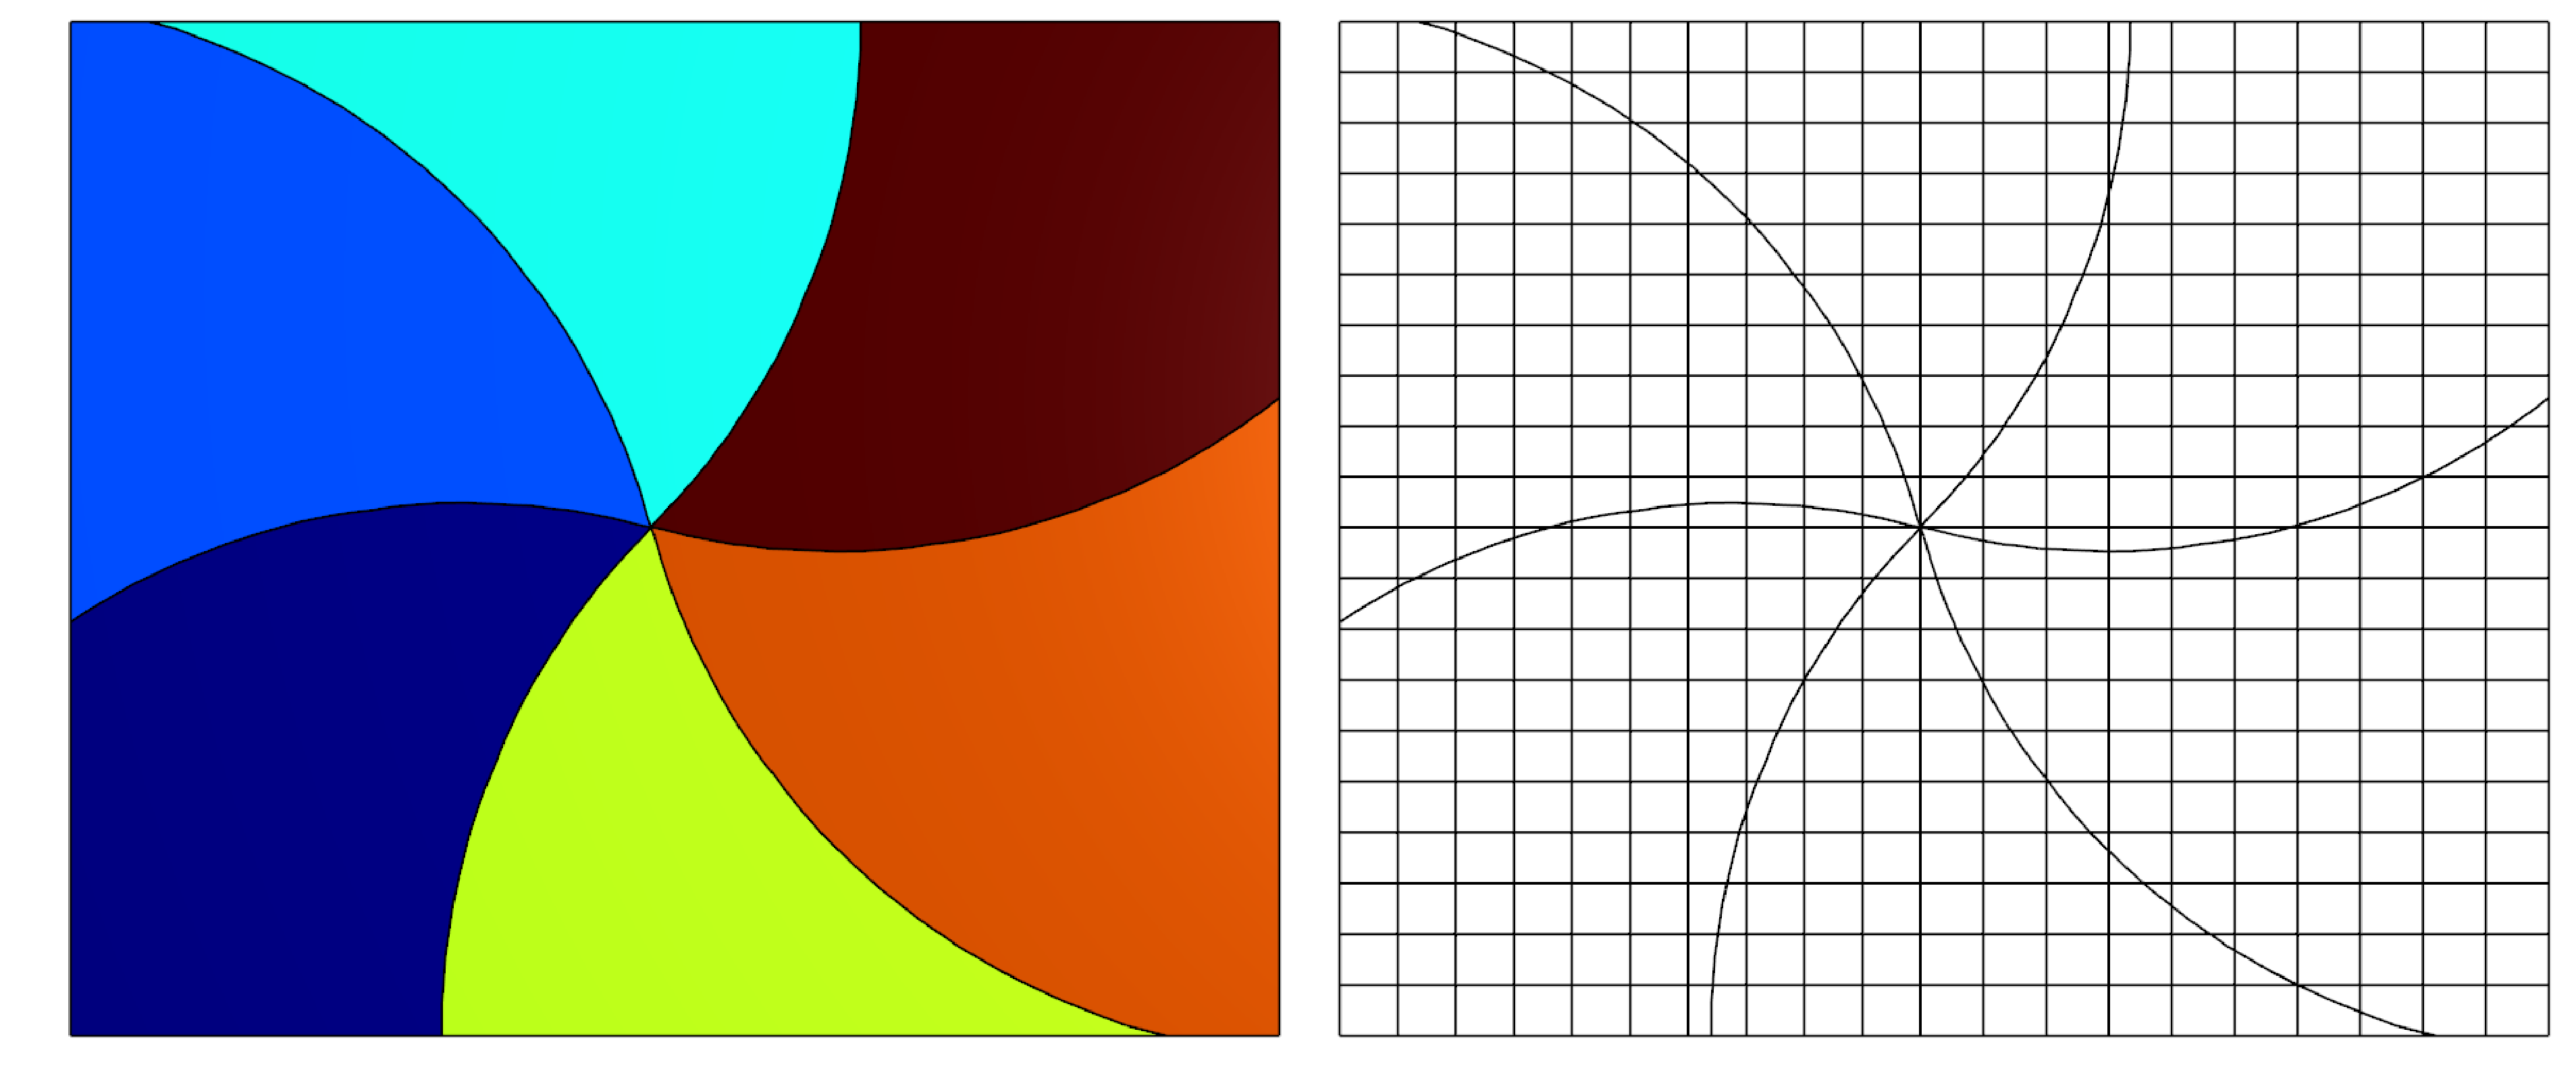
\includegraphics[width=0.8\linewidth]{figures/piecewise_dog_from_crease}
	\caption{Given a crease pattern, we create a separate DOG for each segment (see the different colors) and use the boundary constraints as in \cite{rabi2018shape}. \OSH{Color the crease curves on the right in dark blue, same as in previous figures.}}
	\label{fig:piecewise_dog_from_crease}
\end{figure}

\begin{figure} [h]
	\centering
	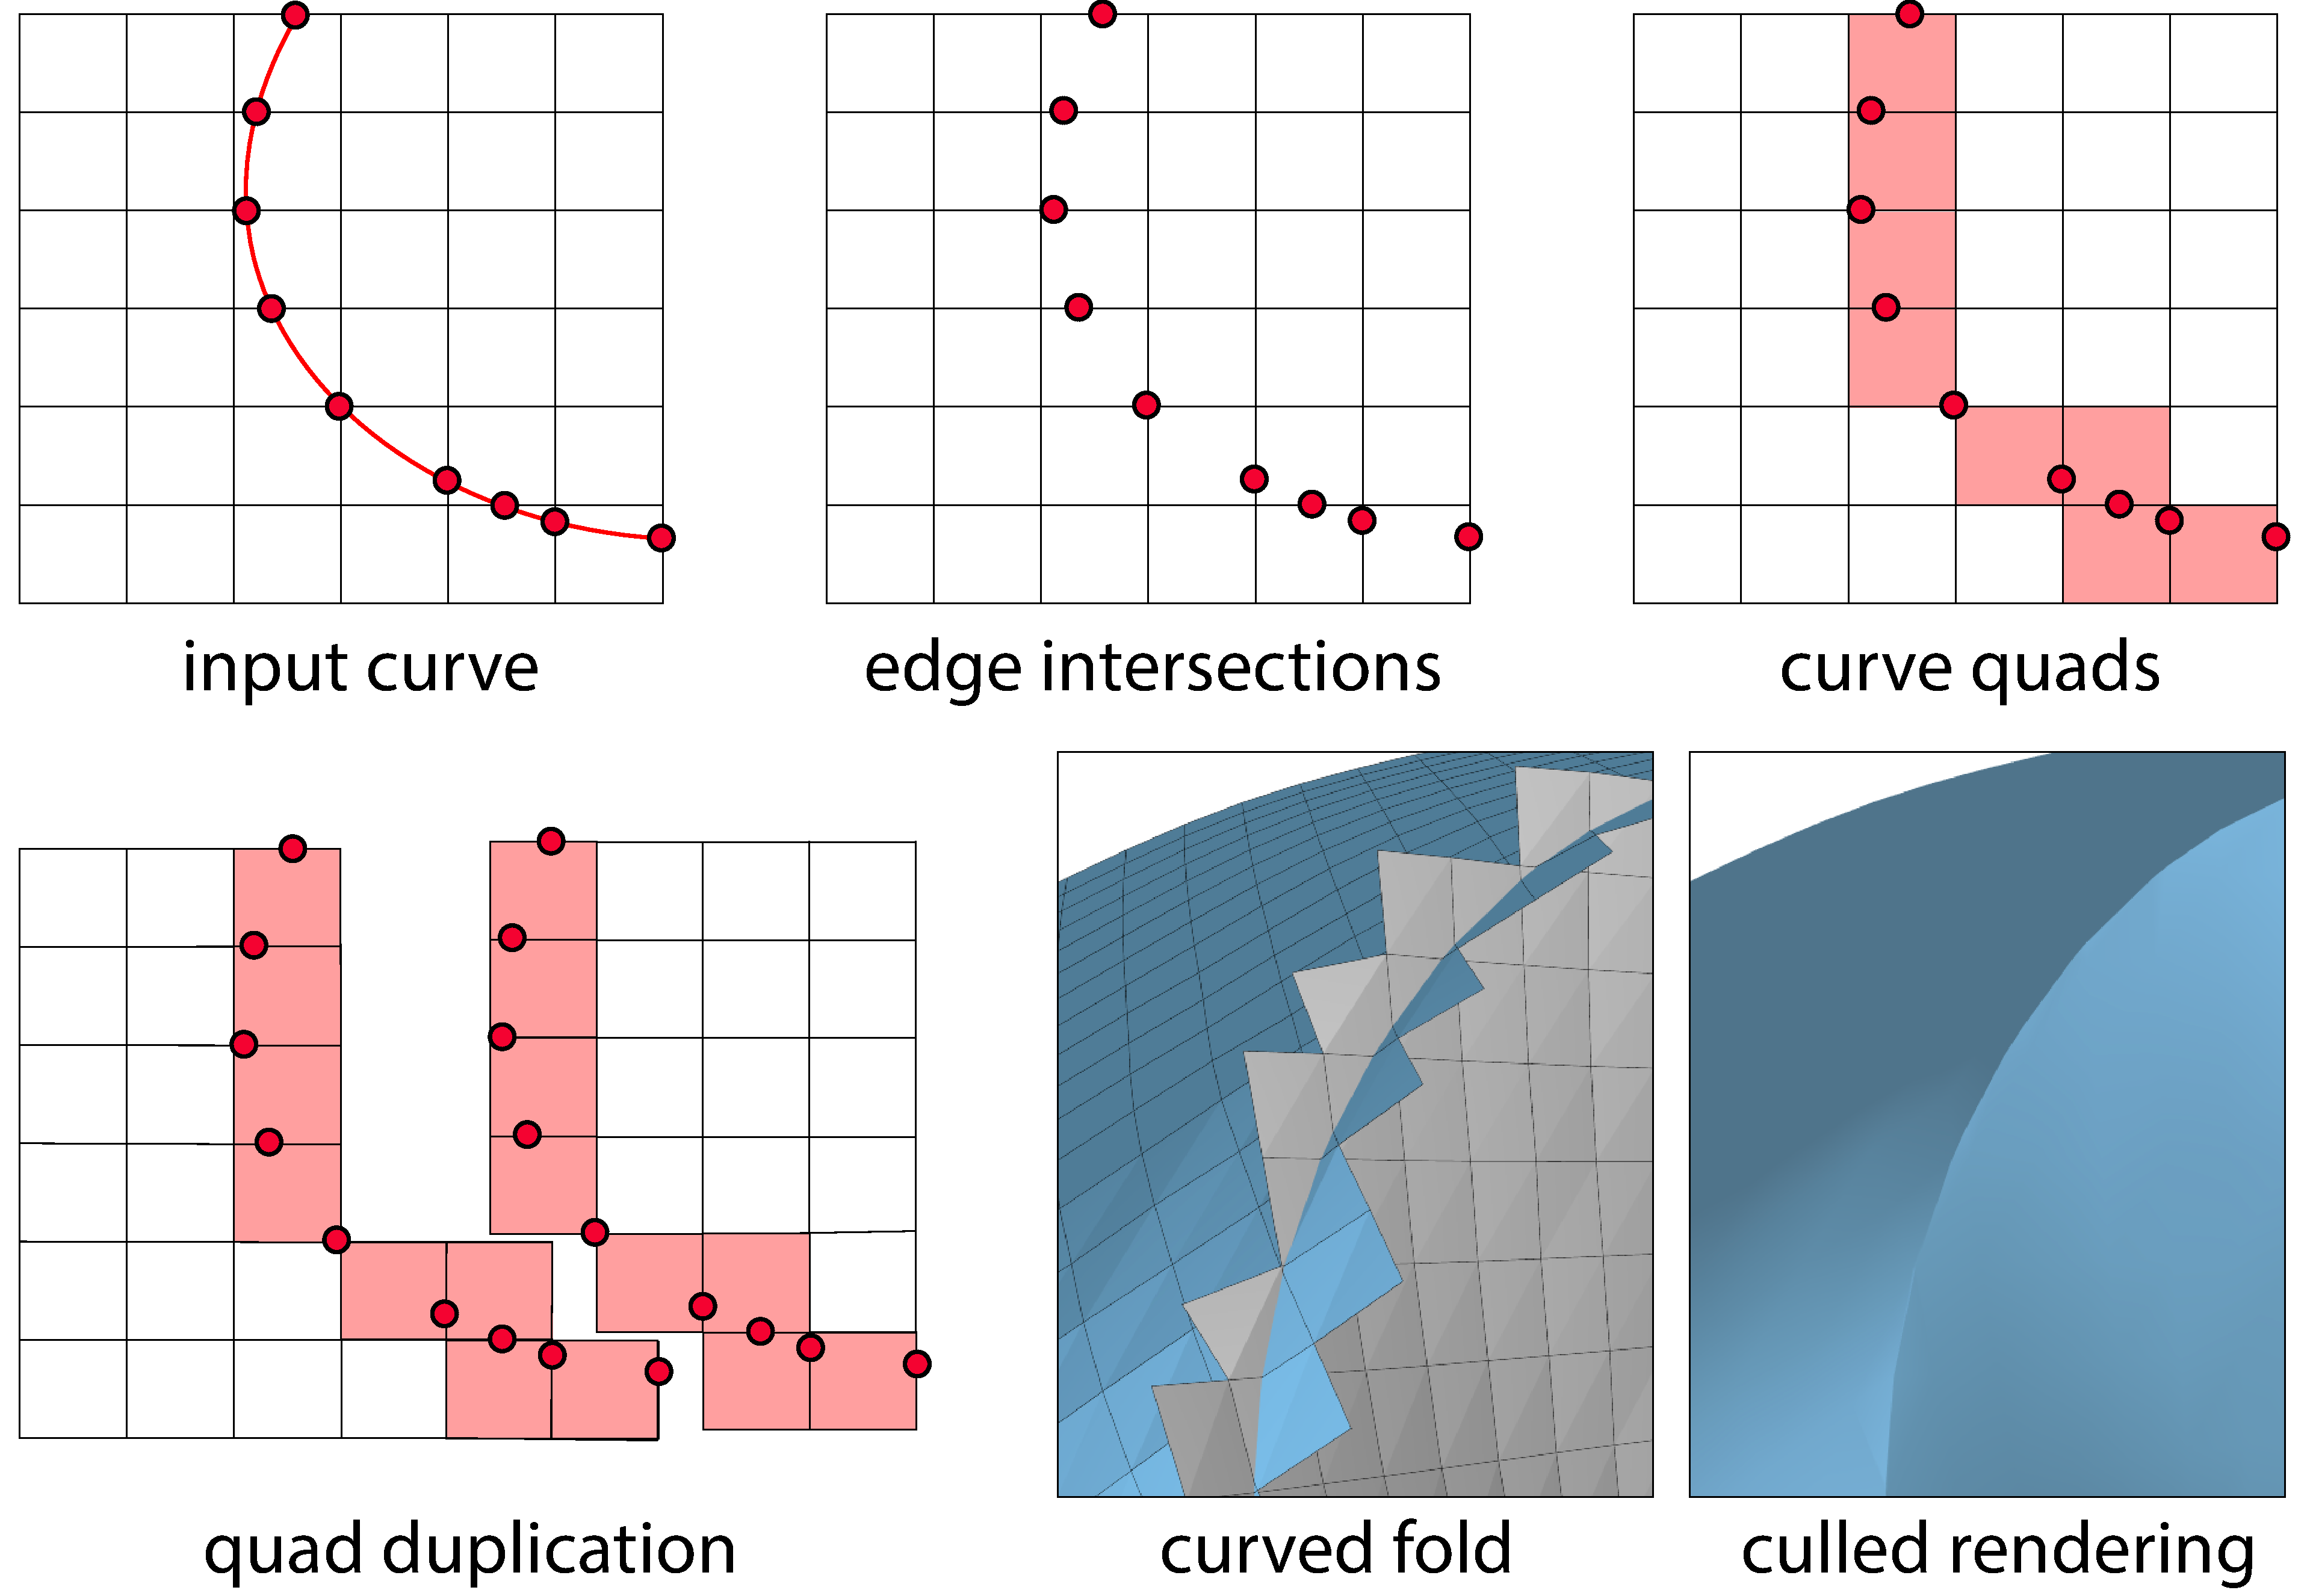
\includegraphics[width=0.8\linewidth]{figures/curve_on_dog}
	\caption{Picture taken from \cite{rabi2018shape}. \OSH{I would redo so it doesn't look like self-plagiarism, with several curves (two?) meeting at a crease vertex. Can be a t-junction to avoid too much clutter. "input" could be just the boundary and the curves, no grid and no points on the curves. Then plot the grid, saying that we pass grid lines through crease vertices. Then show the split view, all patches separated ("quad duplication"), and in that subfigure also show the intersection points of the curve with the grids. The rest can be similar. I maintain that grey+blue looks weird, as if the grey patch is inverted normals. Maybe using the same blue shading color on both sides of the crease is ok?}}
	\label{fig:curve_on_dog}
\end{figure}

\subsection{Desiderata}
Our goal is to develop tools for the exploration of curved folded shapes on top of piecewise DOGs by means of deformations. Our choices are guided by the following ground rules for deforming DOGs:
\begin{enumerate}
  \item Perform homotopy based optimization \label{homotopy_opt}
  \item Minimally constrain DOGs \label{minimal_const}
%  \item Use accurate functionals \label{accurate_func}
%  \item Use simple functionals
\end{enumerate}
\textbf{Homotopy based optimization} is motivated both theoretically and empirically; Modeling DOGs requires solving highly constrained and non linear optimization problems, yet the theory of DOGs guarantees the existence of nearby solutions if one starts at a feasible point. In fact, generally the shape space of DOGs is a smooth manifold \cite{rabi2018shape}. This observation is worthwhile in practice; DOGs exploration was demonstrated to perform well using smooth flow, or homotopy based optimization methods both for handle based editing tasks as well for more complicated deformations such as curve-constraining flows \cite{rabi2018shape} (see \figref{fig:homotopy_curve}).
\begin{figure} [h]
	\centering
	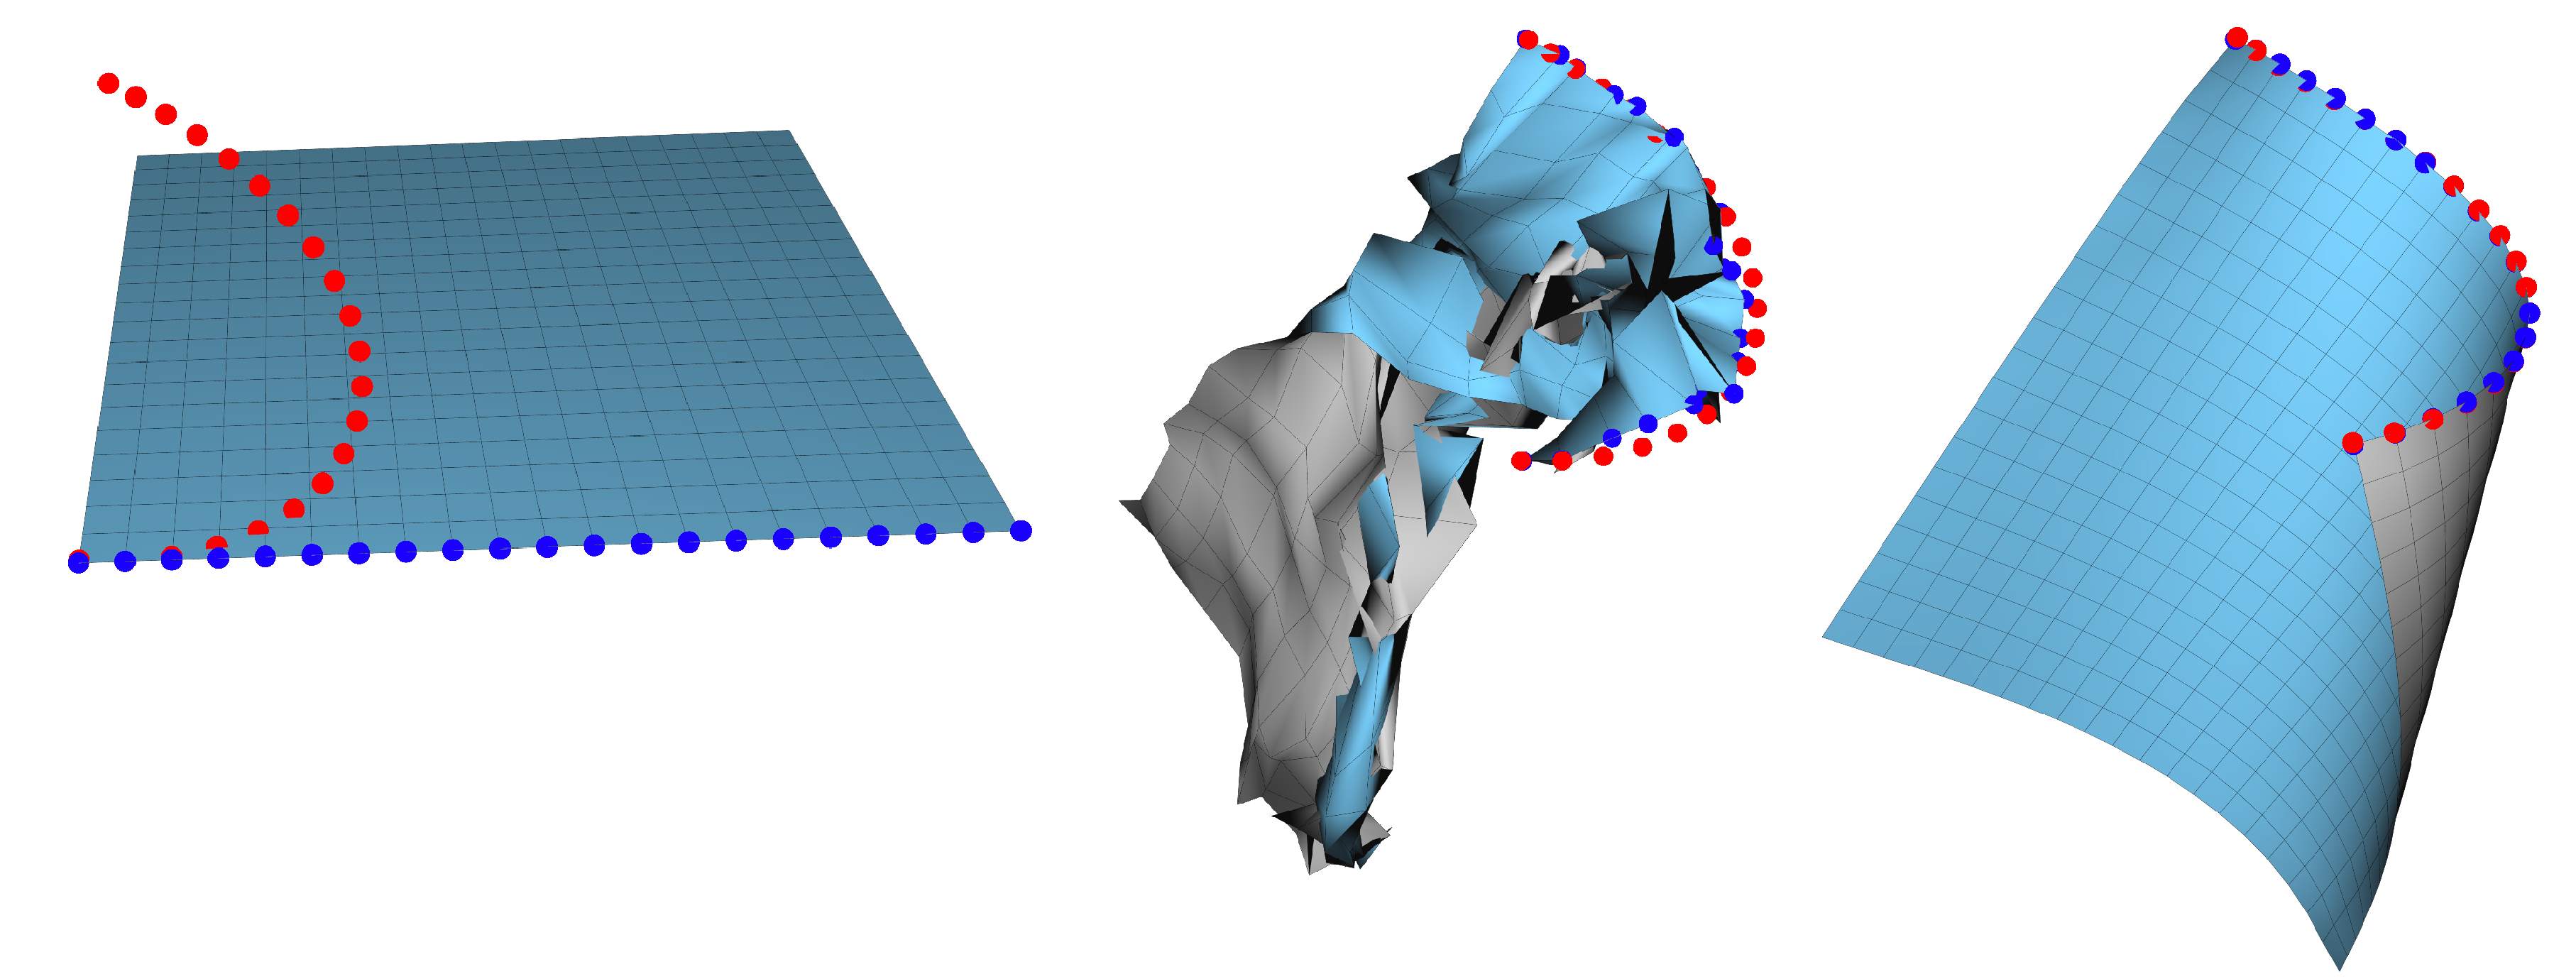
\includegraphics[width=0.8\linewidth]{figures/homotopy_curve}
	\caption{Left: Setting soft positional constraints on a curve of a surface. The same optimization algorithm fails completely when setting all constraints at once, returning a mesh that does not satisfy the non-linear DOG constraints (center) while using a \textit{curve-constraining flow} \cite{rabi2018shape} returns a smooth DOG (right). The latter approach is an homotopy based method that interpolate the positional constraints.} 
	\label{fig:homotopy_curve}
\end{figure}
\\
\textbf{Minimally constrain DOGs.} As DOGs are already heavily constrained, one needs to carefully choose which quantities to constrain by hard constraints, and which ones should be optimized using soft constraints. This is essential to avoid locking, or ill-posed problems in case the constraint gradients are linearly independent \cite{rabi2018shape}. In particular, the rigidity analysis in \cite{rabi18} demonstrates that one cannot fix all edge length exactly, or likewise demand a DOG to also be a Chebyshev net. We note however that this can be done approximately and to a low tolerance as a DOG is a chebyshev at the smooth limit and at the smooth limit there is a rich set of exact isometries. The folding constraints at \secref{sec:folding} where chosen such that they could be satisfied \textit{exactly}, while also vanishing once the surface is sufficiently folded, just like a piecewise smooth curved folded surface. \\
%\textbf{Accurate functionals.} We look for constraints and objectives that are accurate and as often in the case with DOG objectives, converge under sampling of a smooth orthogonal geodesic net \cite{rabi18,rabi2018shape}. \\
%\textbf{Simple functionals.} We strongly prefer sparser objectives with a lower degree as possible. To that end, we leverage the regularity of the DOG meshing and theory on smooth orthogonal geodesic nets in our derivations. \\